\documentclass [10 pt, a4 paper]{article}
\usepackage{booktabs}
\usepackage[utf8]{inputenc}
\usepackage{graphicx}
\usepackage{array}
\usepackage{caption} % for \captionof
\usepackage{amsmath}
\author{Vincent Richard}
\date{02/11/17}
\title{Computtional Methods and C++ Assigment}
\setlength\parindent{24pt}

\begin{document}

\begin{titlepage}
    \maketitle
\end{titlepage}
\newpage

\begin{abstract}
    Sample text
\end{abstract}

\tableofcontents
\listoffigures
\listoftables
\newpage

%%%%%%%%%%%%%%%%%%%%%%%%%%%%%%%%%    Introduction    %%%%%%%%%%%%%%%%%%%%%%%%%%%%%%%%%%%%%%%%%

\section{Introduction}

In this assignment we are asked to examine the application of numerical schemes
for the solution of partial diferential equations. In order to  do so we will consider 
the following probem.

A wall 1 ft. thick and infinite in other directions has an initial uniform temperature Tin of 100$^{\circ}$F. The surface temperatures Tsur at the two
sides are suddenly increased and maintained at 300$^{\circ}$F. The wall is composed of
nickel steel (40\% Ni) with a diffusivity of D = 0:1 ft2=hr. Please compute the
temperature distribution within the wall as a function of time.
The governing equation to be solved is the unsteady one-space dimensional
heat conduction equation, which in Cartesian coordinates is:
\begin{equation}
    \frac{\partial T}{\partial t} = D \frac{\partial T}{\partial x^{2}}
\end{equation}

\subsection{Presentation of the different methods used}

\subsubsection{DuFort-Frankel}
The DuFort-Frankel scheme is an explicit scheme unconditionnaly stable the parabolic PDE is:
\begin{equation}
    \frac{T_{i}^{n+1} - T_{i}^{n-1}}{2\Delta t} = D \frac{T_{i+1}^{n} -(T_{i}^{n+1} + T_{i}^{n-1}) + T_{i-1}^{n})}{\Delta x^{2}}
\end{equation}
This equation leads to an explicit form which is:
\begin{equation}
    T_{i}^{n+1}(1 + 2r) = T_{i}^{n-1} +2r(T_{i+1}^{n} - T_{i}^{n-1} + T_{i-1}^{n}), r =\frac{D\Delta t}{\Delta x^{2}}
\end{equation}

\subsubsection{Richardson}
The Richardson scheme is an explixit scheme, unconditionnaly unstable:
\begin{equation}
    \frac{T_{i}^{n+1} - T_{i}^{n-1}}{2\Delta t} = D \frac{T_{i+1}^{n} - 2 T_{i}^{n} + T_{i-1}^{n}}{\Delta x^{2}}
\end{equation}
This equation leads to an explicit form which is:
\begin{equation}
    T_{i}^{n+1} = 2r(T_{i+1}^{n} - 2T_{i}^{n} + T_{i-1}^{n}) + T_{i}^{n-1}, r=\frac{D\Delta t}{\Delta x^{2}}
\end{equation}
%If we substitute the Fourier  mode $T_{i}^{n} = \lambda_{k}^{n}e^{ik\pi j\Delta x}$ into the scheme we are lead to the characteristic equation of the Richardson scheme:
%\begin{equation}
%    \lambda_{k}^{2}+8\lambda_{k}\mu sin^{2}(\frac{k\pi \Delta x}{2}) - 1 = 0
%\end{equation}

\subsubsection{Laasonen}
The Laasonen scheme is an implicit scheme, that as for equation:
\begin{equation}
    \frac{T_{i}^{n+1} - T_{i}^{n-1}}{2\Delta t} = D\frac{T_{i+1}^{n} - 2T_{i}^{n} + T_{i-1}^{n}}{\Delta x^{2}}
\end{equation}

This equation leads to a form that result in asystem of linear equation:
\begin{equation}
    -r T_{i+1}^{n+1} + (1+2r)T_{i}^{n+1} -rT_{i-1}^{n+1} =T_{i}^{n}, r=\frac{D\Delta t}{\Delta x^{2}}
\end{equation}

\subsubsection{Cranck-Nicholson}
The Crank-Nicholson scheme is an implicit scheme, that as for equation:
\begin{equation} 
    \frac{T_{i}^{n+1} - T_{i}^{n}}{\Delta t} = \frac{D}{2}(\frac{T_{i+1}^{n+1}-2T_{i}^{n+1}+T_{i-1}^{n+1}}{\Delta x^{2}} + \frac{T_{i+1}^{n}-2T_{i}^{n}+T_{i-1}^{n}}{\Delta x^{2}})
\end{equation}

This equation leads to a form that result in asystem of linear equation:
\begin{equation}
    -\frac{r}{2} T_{i+1}^{n+1}+(1+r)T_{i}^{n+1}-\frac{r}{2}T_{i-1}^{n+1} = \frac{r}{2}T_{i+1}^{n} + (1-r)T_{i}^{n} + \frac{r}{2}T_{i-1}^{n}
\end{equation}
\quad

%%%%%%%%%%%%%%%%%%%%%%%%%%%%%     Methods Procedures      %%%%%%%%%%%%%%%%%%%%%%%%%%%%%%%%%%%%%

\section{Methods and Procedures}

    To resolve the problem we decided to create a Oriented Object program base on 
those figures (for readibility reason I divided the structure in three graphics):
\begin{center}
    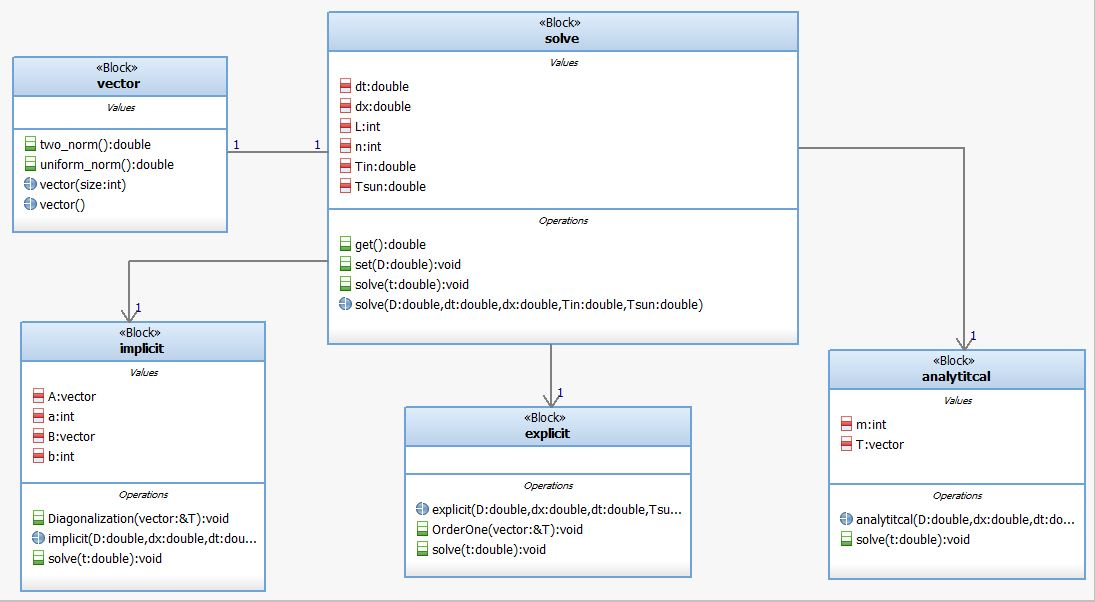
\includegraphics[scale=0.6]{Chart/General.JPG}
    \captionof{figure}{General Architecture}
\end{center}
%%%%%%%%%%%%% Solve
The based class is \textbf{Solve}. It has a number of argument:
\begin{itemize}
    \item D the diffusivity which is in the assigment of $D = 0.1$  \textit{$ft^{2}$/hr}
    \item dt the gap in time between n and n+1
    \item dx the gap in space between i and i+1
    \item Tin the initial temperature of the wall here $Tin = 100^{\circ}F$
    \item Tsun the temperature on the two sides that are maintained at $Tsun = 300^{\circ}F$
    \item L the lenght of the wall which is fix to 1 ft. in this exercice
    \item n the number of possible position x for a fixed t, it calculated with $n = \frac{L}{dx}$
\end{itemize}

\vspace{0.3cm}
It also has couples of methods:
\begin{itemize}
    \item Solve(double D, double dx, double dt, double Tsun, double Tin), the only constructor of 
    this class and initialize the different value depending on the user input
    \item solve(double t) a virtual methods that is created to be use in the derived class it will be the function
    that solve and print the result of the problem.
    \item get() / set() methods, basic accessor methods   
\end{itemize}

\vspace{0.3cm}
The \textbf{Solve} class also have three derived class \textbf{Implicit}, \textbf{Explicit}, and \textbf{Analytical}.
The \textbf{Implicit} and \textbf{Explicit} class are further details below. We will talk about the \textbf{Analytical} class.
%%%%%%%%%%%%%%%% Analytical
\vspace{0.3cm}

The class \textbf{Analytical} calculate the analytical solution of the input problem.
The class provided two new arguments:
\begin{itemize}
    \item m it is an integer used to simplify the expression of T since the anatical value of T is : 
    \begin{equation}
        T = T_{sur} + 2(T_{in}-T_{sur}) \sum_{m=1}^{m=\infty} e^{-D(m\pi /L)^{2}t} \frac{1-(-1)^{m}}{m\pi} sin(\frac{m\pi x}{L})
    \end{equation}

    So we need to get a smaller m for the upper border of the sum. We choosed to fix it at 10 000, 
    the result obtain was close enought to make this simplification.

    \item T it is a vector defined as an argument to initialize it in the constructor
\end{itemize}
The \textbf{Analytical} class has also two methods :
\begin{itemize}
    \item The constructor analytical(...) it is based on the constructor of the solve class, it also
    initialize the value of m and the vector T
    \item The solve function that is here defined to print the value of the analytical solution T 
    of the problem with the approximation as explain above. It will print the value of T at each 0.1hr
    until the argument t is reach
\end{itemize}

%%%%%%%%%%%%%%%% Vector
\vspace{0.3cm}

The \textbf{Vector} class is associated with the \textbf{Solve} class, it is use to defined 
vector in the derived class.
The methods of the vector class:
\begin{itemize}
    \item one\_norm
    \item two\_norm
    \item uniform\_norm
\end{itemize}
are used to compare the analytical and the different schemes methods.

%%%%%%%%%%%%%% Explicit
\begin{center}
    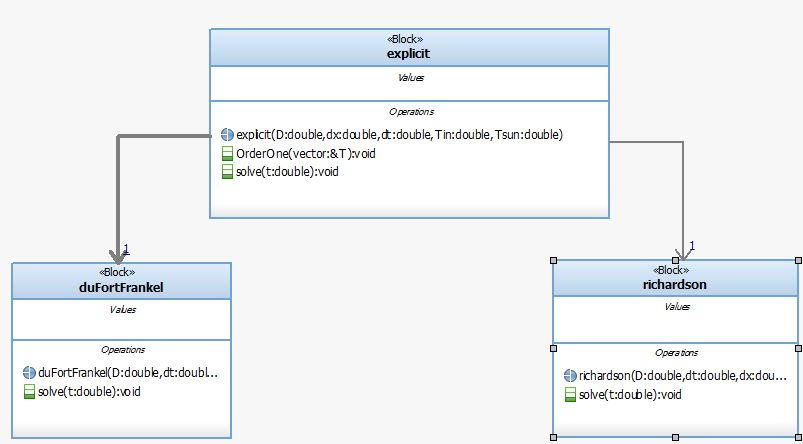
\includegraphics[scale=0.6]{Chart/Explicit.JPG}
    \captionof{figure}{Explicit Architecture}
\end{center}

The derived \textbf{Explicit} class is also a based class for two other class: the \textbf{DuFortFrankel}
class and the \textbf{Richardson} class. Each of them solving the problem with the scheme of the same name.

\vspace{0.3cm}

The \textbf{Explicit} class doesn't define any new argument and as the same methods has the \textbf{Solving}
class. But it does define an aditionnal method. 

The \textbf{OrderOne} method was created because in the two explicit schemes, DuFort-Frankel
and Richardson, we encounter the issue of not being able to start the scheme at $n = 1$.
To find a the value of the temperature T at a time n we need the value of T at n and n-1 (See equation (3) and (5))>.
The problem set the values of T at $n = 0$ but we still need to find T at $n=1$ to use those
schemes. So we first need the method \textbf{OrderOne} to find T at $n = 1$ with a forward time central
space scheme, and then apply the Richardson and DuFort-Frankel scheme to find the other values 
of T.

Since this method is useful for both derived class, we decided to declare it in the 
\textbf{Explicit} class.

\vspace{0.3cm}

The two derived classes \textbf{DuFortFrankel} and \textbf{Richardson} work the same way.

They have the same constructor method based on the one defined in the \textbf{Explicit} class
and they both defined the method \textbf{solve} in a very similar way. 

Once the initialisation of T at $n = 0$ and $n = 1$ (with the \textbf{OrderOne} method) 
is done, we use a loop on depending on the scheme the equation (3) or (5) until we reach 
the value of t wanted by the user.
%%%%%%%%%%%%%%%%% Implicit

\begin{center} 
    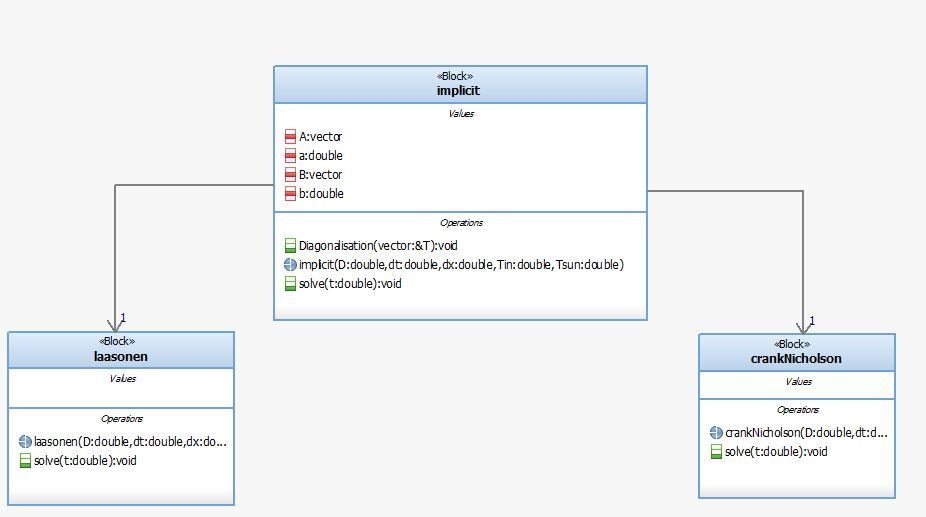
\includegraphics[scale=0.6]{Chart/Implicit.JPG}
    \captionof{figure}{Implicit Architecture}
\end{center}

\vspace{0.3cm}

The derived \textbf{Implicit} class is also a based class for two other class: the 
\textbf{Laasonen} class and the \textbf{Cranck-Nicholson} class. Each of them solving 
the problem with the scheme of the same name.

The \textbf{Implicit} class just like the \textbf{Explicit} as a particular method to 
simplify the solving of the problem in the two derived classes. To understand what the 
\textbf{Diagonalization} method is used for we need to talk about
the resolution of the problem for the two implicit schemes.

\vspace{0.3cm}

The two system of equation that we wrote in equation (7) and (8) can be written like this:

\begin{equation}
\begin{pmatrix} b    &    a   &    0   & \cdots &   0    \\
a    & \ddots & \ddots & \ddots & \vdots \\
0    & \ddots & \ddots & \ddots &    0   \\
\vdots & \ddots & \ddots & \ddots &   a    \\ 
0    & \cdots &    0   &   a    &    b   \\
\end{pmatrix}
=
\begin{pmatrix} T_{0}^{n+1} \\ 
\vdots \\ 
T_{imax}^{n+1} \\
\end{pmatrix}
R
\end{equation}
Where a, b are doubles and P a vector, all of their values change depending on 
which scheme we choose. Since the problem is a tri-diagonal matrix and for each scheme,
we have (in the special case of the data given by the assigment) 
$ 2\left \| a \right \| \leq \left \| b \right \| $ so we can use Thomas algorithm to
solve those equation.

Thomas Algorithm is an efficient way of solving tridiagonal matrix systems. It is based
on LU decompositionin which the matrix system $Mx = r$ is rewritten as $LUx = r$ where L 
is a lower triangular matrix and U is an upper triangular matrix. The system can be 
efficiently solved by setting $Ux = p$ and then solving first $Lp = r$ for p and then 
$Ux=p$ for x. The Thomas algorithm consist of two steps. In step one decomposing the matrix
into $M=LU$ and solving $Lp=r$ are accomplished in a single downwards sweep, taking us
straight from $Mx=r$ to $Ux=p$. In step two the equation $Ux=p$ is solved for x in  an
upward sweep.

In the \textbf{Diagonalization} we are taking care of the first step of the Thomas algorithm.
We will have this kind of equation at the end of the method:

\begin{equation}
\begin{pmatrix} 1    &    B_{0}    & \cdots &   0    \\
                0    & \ddots     & \ddots  & \vdots \\
                \vdots & \ddots & \ddots & B_{imax - 1}  \\ 
                0    & \cdots   &   0    &    1   \\
\end{pmatrix}
=
\begin{pmatrix} T_{0}^{n+1} \\ 
\vdots \\ 
T_{imax}^{n+1} \\
\end{pmatrix}
P
\end{equation}
The values of $B_{i}$ and P will be stored respectively in the B vector and the A
vector defined in the \textbf{Implicit} class.

The function \textbf{solve} in both \textbf{Cranck-Nicholson} and \textbf{Laasonen} 
is a loop that initialize the vector R (with the help of the equation (7) and (9),
call the method \textbf{Diagonalization(R)} and then calculate the second step of the
Thomas algorithm. It will print for each 0.1hr the value of T until the argument t of
solve is reached.
\quad
%%%%%%%%%%%%%%%%%%%%%%%%%%%%%%%%%%%%%%            RESULT             %%%%%%%%%%%%%%%%%%%%%%%

\section{Result}





\end{document}